\documentclass{article}

\usepackage{graphicx}
\usepackage{tikz}
\usepackage{tikzsymbols}
\usetikzlibrary{calc,patterns,shapes.geometric}
\pagestyle{empty}
\usepackage[margin=0pt]{geometry}
\geometry{papersize={14in,12in}}

\def\centerarc[#1](#2)(#3:#4:#5){\draw[#1] ($(#2)+({#5*cos(#3)},{#5*sin(#3)})$) arc (#3:#4:#5);}

\begin{document}
	\begin{figure}
		\centering
		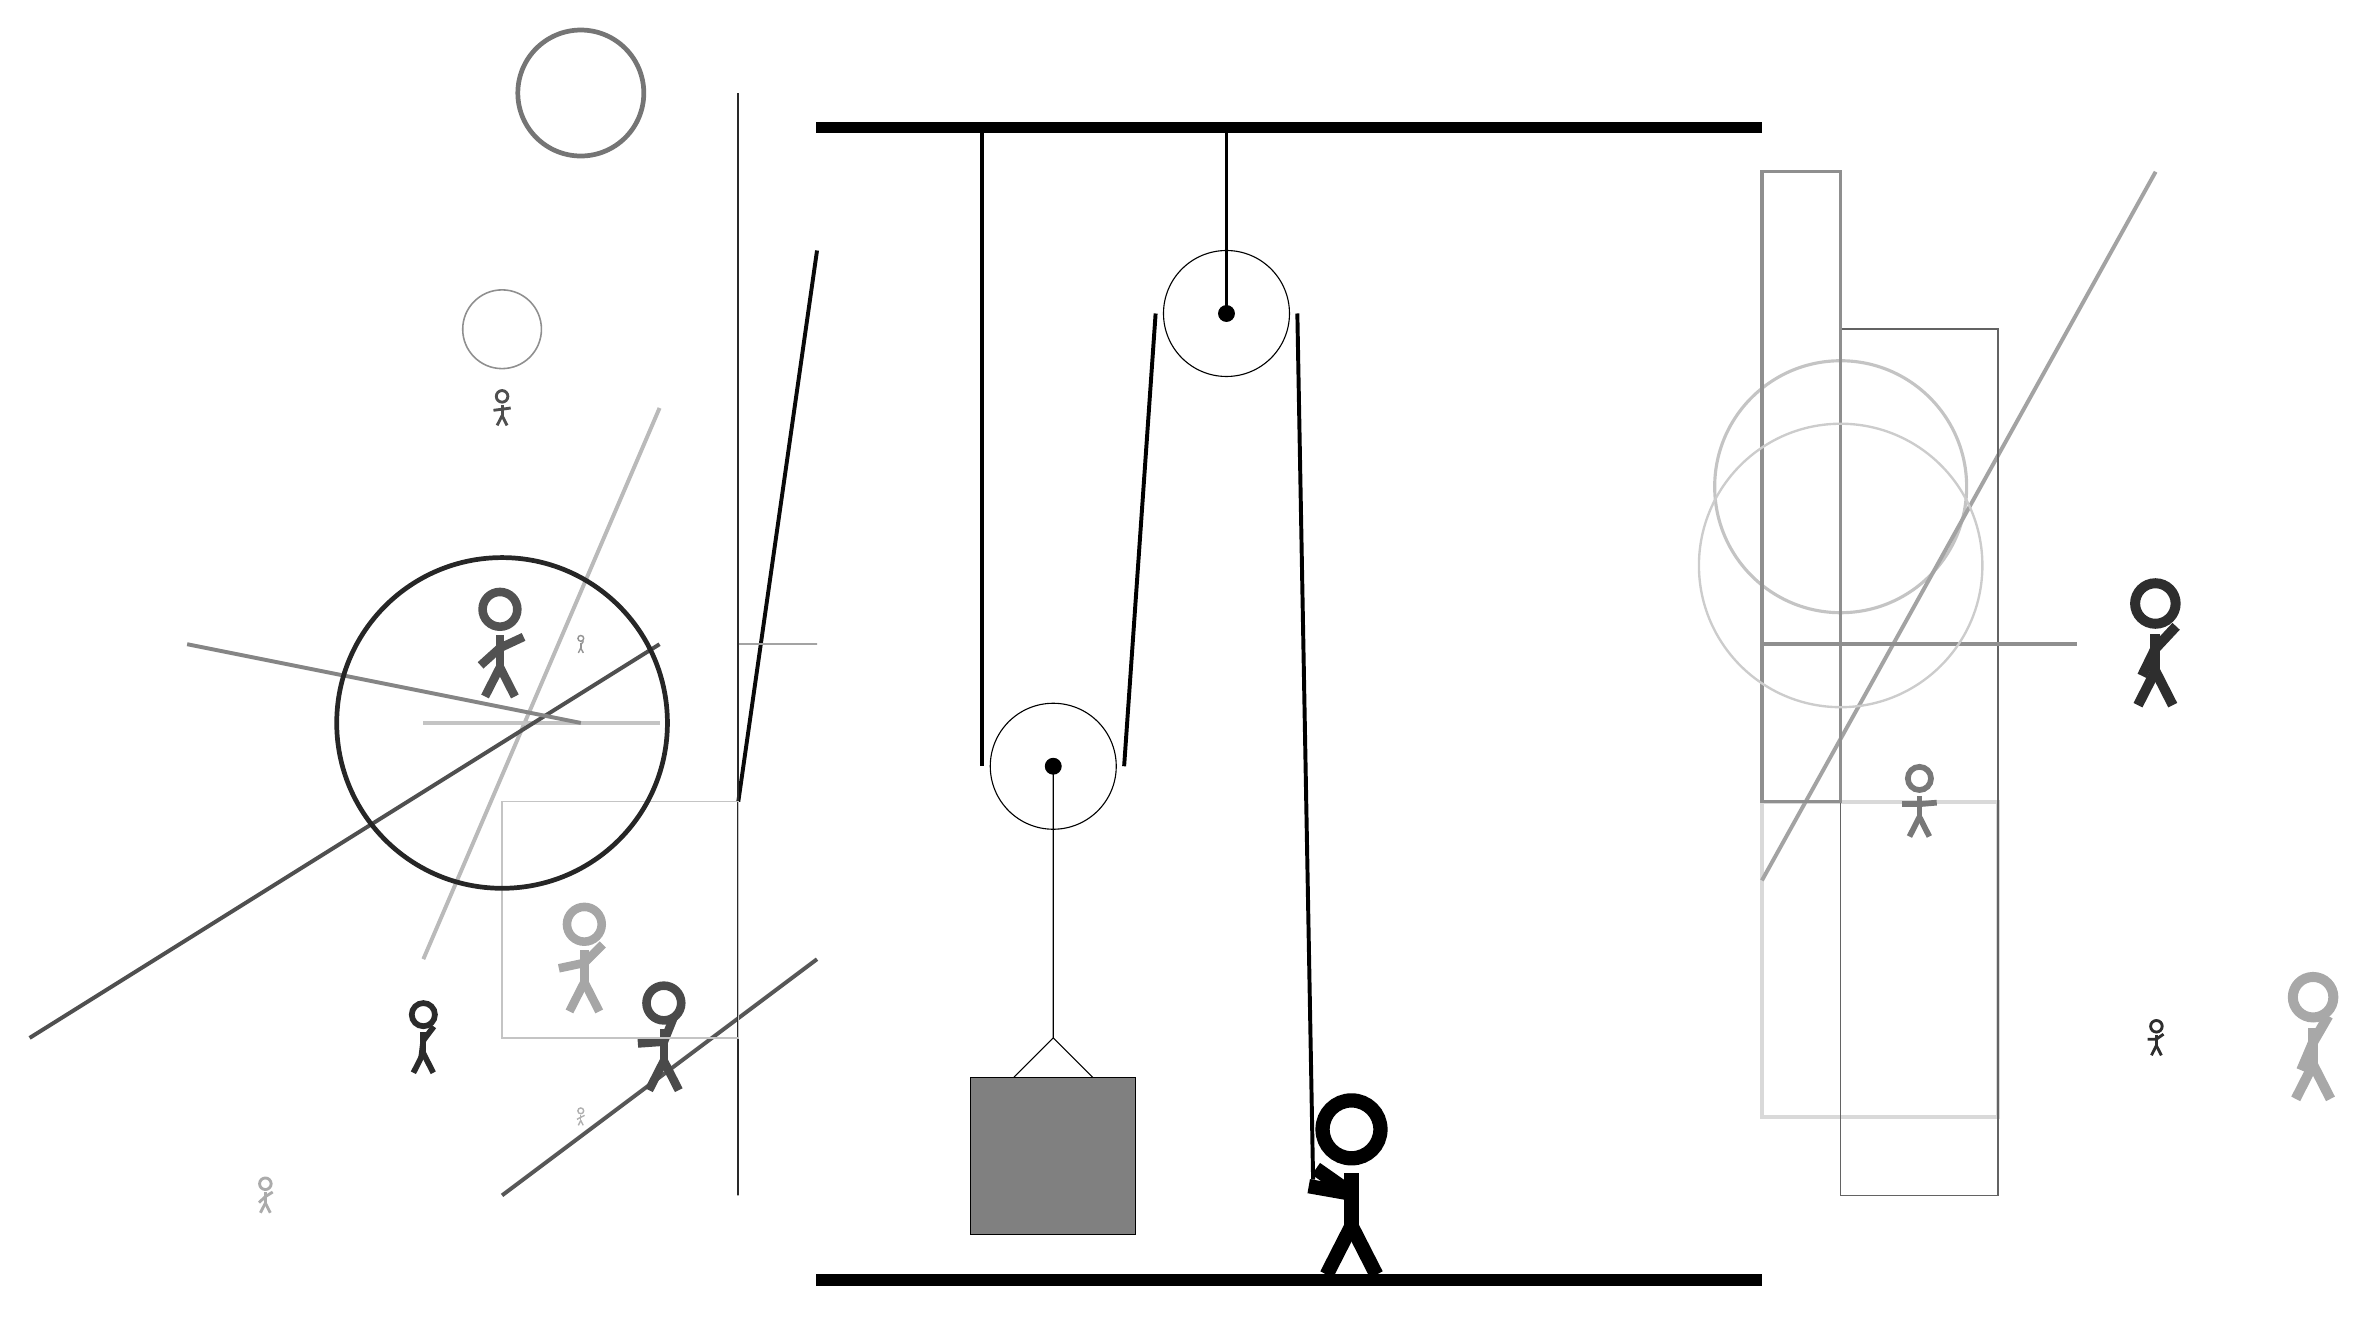
\begin{tikzpicture}
			%%%%% START %%%%%
			
			\draw[fill=black] (-2, 11.5) rectangle (10, 11.625);
			
			\draw (3.2, 9.2) circle (0.8);
			\draw[fill=black] (3.2, 9.2) circle (0.1);
			\draw[thick] (3.2, 9.2) -- (3.2, 11.5);
			
			\draw (1, 3.45) circle (0.8);
			\draw[fill=black] (1, 3.45) circle (0.1);
			
			\draw (1, 3.45) -- (1, 0.0) -- (0.5, -0.5);
			\draw (1, 0.0) -- (1.5, -0.5);
			\draw[fill=black!50] (-0.05, -0.5) rectangle (2.05, -2.5);
			
			\draw[line width=0.5mm] (0.1, 11.5) -- (0.1, 3.45);
			\centerarc[line width=0.5mm](1, 3.45)(180:360:0.9);
			\draw[line width=0.5mm](1.9, 3.45) -- (2.3, 9.2);
			\centerarc[line width=0.5mm](3.2, 9.2)(0:180:0.9);
			\draw[line width=0.5mm](4.1, 9.2) -- (4.3, -1.8);
			
			\draw[line width=0.5mm, color=black!27](-4, 8) -- (-7, 1);
			
			\draw[line width=0.5mm, color=black!15] (10, -1) rectangle (13, 3);
			\draw[line width=0.5mm, color=black!23](-4, 4) -- (-7, 4);
			\draw [line width=0.4mm, color=black!23](11, 7) circle (1.6);
			\draw[line width=0.5mm, color=black!36](10, 2) -- (15, 11);
			\draw [line width=0.6mm, color=black!54](-5, 12) circle (0.8);
			\node[line width=0.3mm, color=black!83] at (-7, 0) {\Strichmaxerl[4][83][53]};
			
			\node[line width=0.5mm, color=black!53] at (12, 3) {\Strichmaxerl[4][0][5]};
			\draw[line width=0.5mm, color=black!96](-2, 10) -- (-3, 3);
			\draw[line width=0.2mm, color=black!61] (11, -2) rectangle (13, 9);
			\node[line width=0.3mm, color=black!31] at (-5, -1) {\Strichmaxerl[1][29][26]};
			\draw[line width=0.5mm, color=black!66](-2, 1) -- (-6, -2);
			\draw[line width=0.4mm, color=black!44] (11, 3) rectangle (10, 11);
			
			\draw [line width=0.2mm, color=black!44](-6, 9) circle (0.5);
			\node[line width=0.6mm, color=black!68] at (-6, 5) {\Strichmaxerl[6][42][25]};
			\node[line width=0.2mm, color=black!33] at (-9, -2) {\Strichmaxerl[2][43][32]};
			\node[line width=0.6mm, color=black!82] at (15, 0) {\Strichmaxerl[2][1][35]};
			\draw[line width=0.5mm, color=black!69](-4, 5) -- (-12, 0);
			\draw[line width=0.2mm, color=black!36] (-2, 5) rectangle (-3, 5);
			\node[line width=0.6mm, color=black!35] at (-5, 1) {\Strichmaxerl[6][12][45]};
			\draw[line width=0.5mm, color=black!44](10, 5) -- (14, 5);
			
			\draw[line width=0.5mm, color=black!48](-5, 4) -- (-10, 5);
			\draw [line width=0.3mm, color=black!20](11, 6) circle (1.8);
			\draw[line width=0.3mm, color=black!84] (-3, 12) rectangle (-3, -2);
			\node[line width=0.7mm, color=black!82] at (15, 5) {\Strichmaxerl[7][64][47]};
			
			\node[line width=0.5mm, color=black!71] at (-4, 0) {\Strichmaxerl[6][4][68]};
			\draw[line width=0.2mm, color=black!23] (-3, 3) rectangle (-6, 0);
			\draw [line width=0.6mm, color=black!85](-6, 4) circle (2.1);
			\node[line width=0.7mm, color=black!69] at (-6, 8) {\Strichmaxerl[2][7][8]};
			
			\node[line width=0.6mm, color=black!42] at (-5, 5) {\Strichmaxerl[1][88][54]};
			\node[line width=0.4mm, color=black!34] at (17, 0) {\Strichmaxerl[7][67][60]};
			
			
			\node at (4.7, -1.9) {\Strichmaxerl[10][-35][170]};
			
			\draw[fill=black] (-2, -3) rectangle (10, -3.15);
			
			%%%%% END %%%%%
		\end{tikzpicture}
	\end{figure}	
\end{document}